\documentclass[10pt, compress]{beamer}

\usetheme{m}

\usepackage{booktabs}
\usepackage[scale=2]{ccicons}
\usepackage{minted}
\usepackage[normalem]{ulem}

\usemintedstyle{trac}

\title{Компьютерная лингвистика}
\subtitle{}
\date{\today}
\author{Маша Шеянова, masha.shejanova@gmail.com\\
        Саша Ершова, asershova@edu.hse.ru}
\institute{НИУ ВШЭ}


\begin{document}

\maketitle

\begin{frame}[fragile]
  \frametitle{Что такое "компьютерная лингвистика"?}
  Есть лингвистика. Есть компьютеры. Что хорошего можно с этим сделать?
  
  \begin{enumerate}
  \item Можно делать корпуса и вспомогательные инструменты для теоретических лингвистов.
  \item Computational linguistics: изучение языка при помощи формальных математических моделей, статистики и всего такого.
  \item Natural language processing: автоматическое извлечение чего-нибудь из текста и автоматическое его порождение.
  \end{enumerate}
  
  \alert{NB:} 2 и 3 --- очень разные вещи, хотя и то, и другое в русском называют "компьютерной лингвистикой"
\end{frame}
\section{Вспомогательные инструменты}

\begin{frame}[fragile]
  \frametitle{Какие они бывают?}
  \begin{itemize}
  \item Корпуса
  \item Словари
  \item Инструменты сбора данных
  \item Программы для анализа данных (анализ звука: Praat, анализ морфологии: Fieldworks) 
  \end{itemize}
\end{frame}

\begin{frame}
  \frametitle{Сбор данных. Senti game.}
  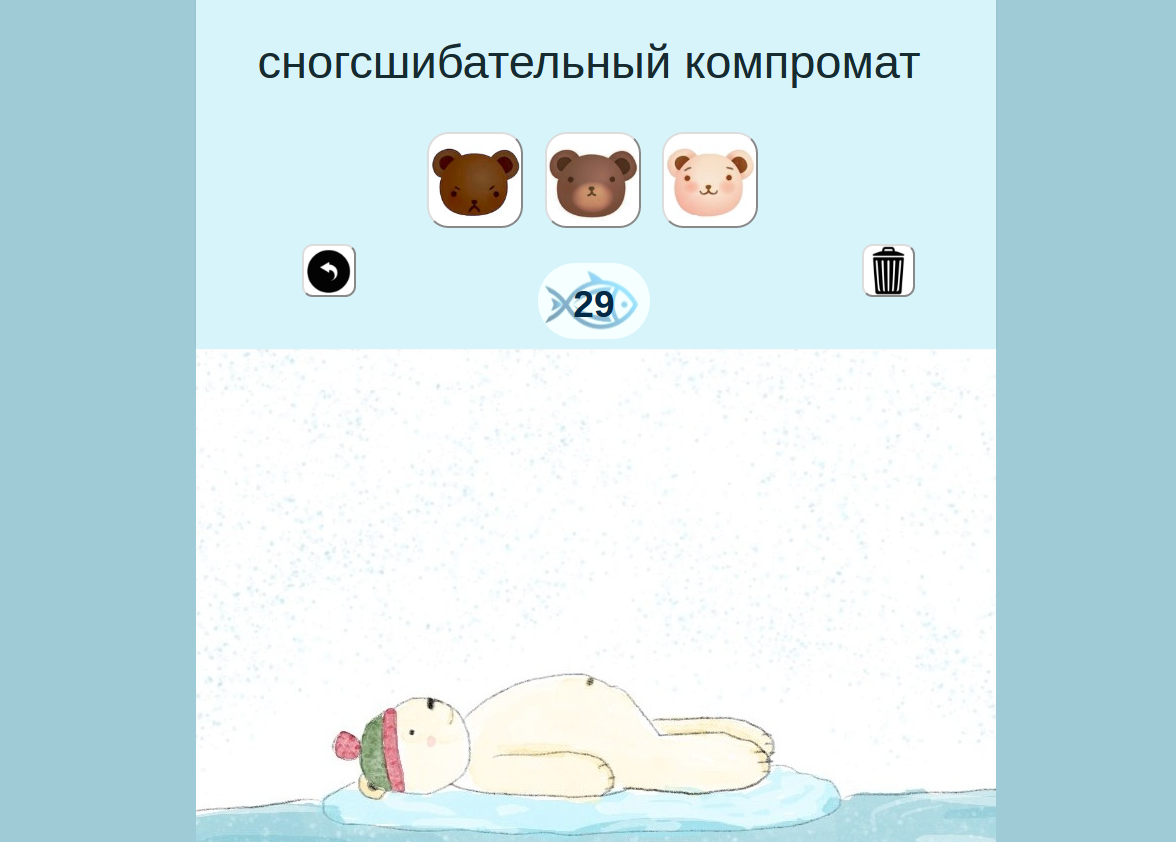
\includegraphics[width=\textwidth]{images/sentinet.png}
\end{frame}

\begin{frame}
  \frametitle{Анализ данных. Praat.}
  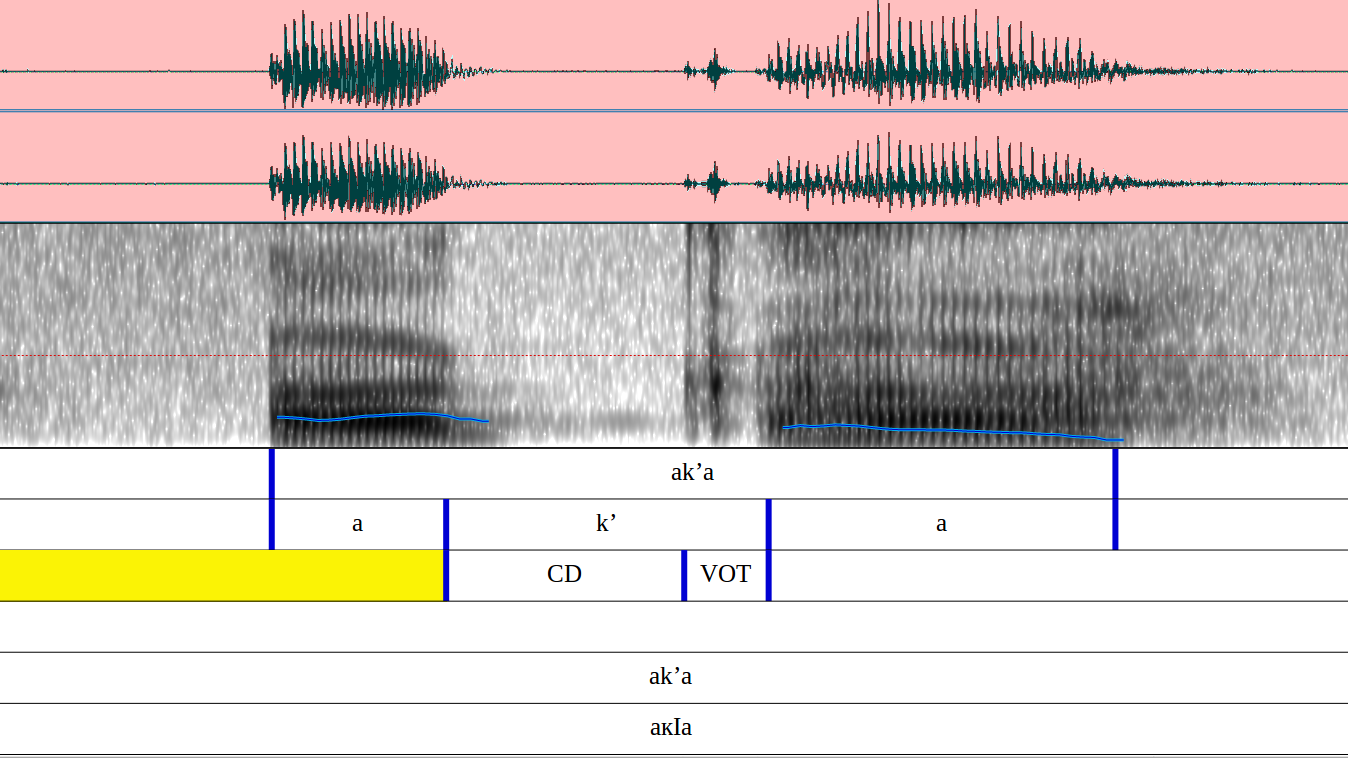
\includegraphics[width=\textwidth]{images/praat.png}
\end{frame}

\section{Computational linguistics}
\begin{frame}
  \frametitle{Что сюда входит?}
  В принципе, это любые лингвистические исследования, где нужно что-то посчитать, например:
  \begin{itemize}
%   \item то, что вы, чуваки, делали на килях с Лизой
  \item посмотреть, от чего возникают дырки в парадигмах
  \item доказать, что вид в русском --- это континуум
  \item посмотреть, какие слова ближе по значению, а какие дальше (этим умеет заниматься дистрибутивная семантика)
  \end{itemize}
\end{frame}

\begin{frame}
 \frametitle{Дистрибутивная семантика. Что это.}
 Что мы хотим:
 \begin{itemize}
 \item формальный способ считать лексическую близость
 \item глобально: научить компьютер извлекать смыслы из текста
 \end{itemize}
 Как делать это автоматически?\\\\
 \alert{Дистрибутивная гипотеза}: значения слов полностью определяются их контекстами. Слова с похожими типичными контекстами имеют схожее значение.
\end{frame}

\begin{frame}
 \frametitle{Дистрибутивная семантика. Как это работает.}
 Нам нужно:
 \begin{itemize}
 \item много текстов, чтобы картинка была репрезентативной
 \item посчитать в этих текстах взаимную встречаемость слов друг с другом
 \item найти слова, которые могут заменить друг друга и слова, у которых нет общих контекстов
 \end{itemize}
 Готово! Мы прекрасны и можем
 \begin{itemize}
 \item находить слова, близкие по значению к данному
 \item строить семантические пропорции
 \item строить семантические визуализации
 \end{itemize}
\end{frame}

\begin{frame}
 \frametitle{Дистрибутивная семантика. Это работает!}
 На \href{http://ling.go.mail.ru/dsm/en/}{rusvectores} можно найти слова, наиболее близкие к данному, построить семантическую пропорцию и многое другое.\\\\
 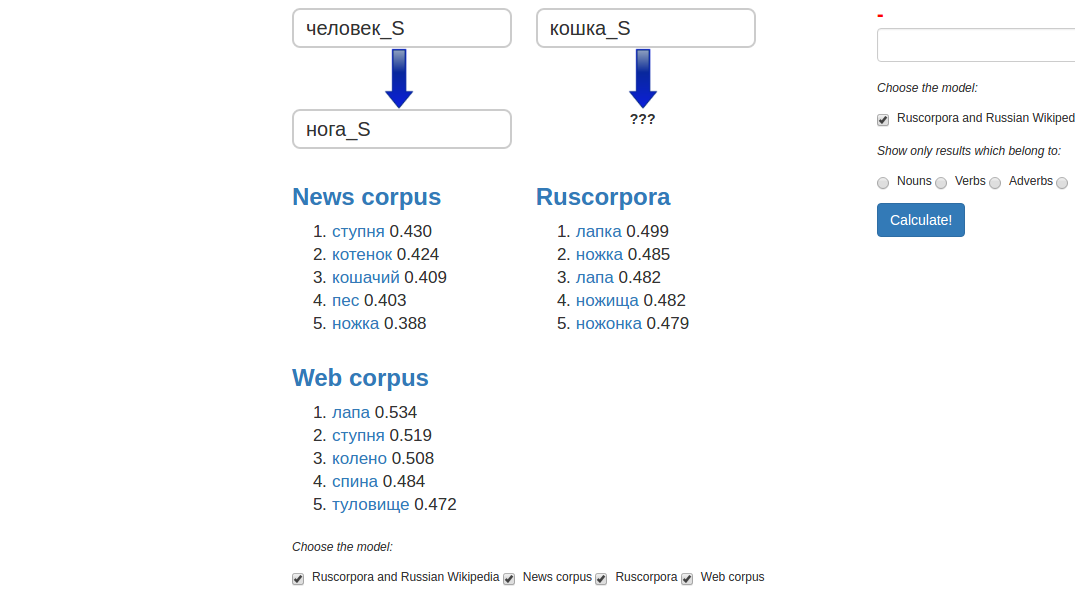
\includegraphics[width=\textwidth]{images/rusvectores.png}
\end{frame}
  
\section{Natural language processing}
\begin{frame}
  \frametitle{Примеры}
  \begin{itemize}
  \item Спеллчекеры
  \item Машинный перевод
  \item Text mining
  \item Speech recognition и OCR
  \item Когнитивные технологии: боты, weak AI, seq2seq-нейросети	
  \end{itemize}
\end{frame}

\begin{frame}
  \frametitle{Машинный перевод. Corpus-based.} 
У нас есть параллельные корпуса, то есть корпуса, где каждое предложение одного языка сопоставлено с предложением другого. С их помощью мы учим компьютер переводить предложения пользователя.
  \begin{table}
    \begin{tabular}{ll}
      Английский & Японский\\
      \toprule
      How much is that red umbrella? & Ano akai kasa wa ikura desu ka.\\
      \midrule
      How much is that small camera? & Ano chiisai kamera wa ikura desu ka.\\
      \bottomrule
    \end{tabular}
  \end{table}
Corpus-based бывает:
\begin{itemize}
\item Statistical
\item Example-based
\end{itemize}
\end{frame}

\begin{frame}
  \frametitle{Машинный перевод. Rule-based.} 
Параллельные корпуса не используются. Часть информации хранится в словарях, часть прописана в правилах.\\\\
Как это работает в Apertium
	\begin{itemize}
	\item словари:
    \begin{itemize}
    	\item билингвальные: лексические соответствия
		\item монолингвальные: парадигмы
	\end{itemize}
    \item правила:
    \begin{itemize}
        \item лексический выбор: сложно → difficult, complicated или complex?
        \item разрешение морфологической омонимии
        \item изменение структуры
    \end{itemize}
    \end{itemize}
\end{frame}

\begin{frame}
  \frametitle{Машинный перевод. Rule-based vs. Corpus-based.} 
  Corpus-based:
  \begin{itemize}
  \item широко используется сейчас (Google, Яндекс)
  \item требует параллельные корпуса: чем больше, тем лучше
  \item в принципе, не требует лингвистических знаний
  \end{itemize}
  Rule-based:
  \begin{itemize}
  \item сейчас всё больше уступает статистическому, \alert{НО}
  \item может применяться при отсутствии больших корпусов → можно работать с малыми языками!
  \item их можно постепенно улучшать
  \item требует лингвистических знаний
  \end{itemize}
\end{frame}

\begin{frame}
  \frametitle{Text mining} 
  Автоматическое извлечение информации для:
  \begin{itemize}
  \item категоризации текстов
  \item информационного поиска
  \item извлечения информации
  \end{itemize}
\end{frame}
  
\begin{frame}
  \frametitle{Speech recognition и OCR}
  OCR --- Optical Character Recognition --- извлечение текста из картинки.
  
  Speech recognition --- извлечение текста из аудиозаписи.
  
  Зачем нам это, если можно просто взять и послушать/почитать?
\end{frame}

\begin{frame}
  \frametitle{Speech recognition и OCR}
  OCR --- Optical Character Recognition --- извлечение текста из картинки.
  
  Speech recognition --- извлечение текста из аудиозаписи.
  
  Зачем нам это, если можно просто взять и послушать/почитать?
  \begin{itemize}
  \item \textbf{Невероятно много информации.} 
  \item Возможность "на лету" проделывать с извлечённым текстом ещё какие-нибудь операции.
  \end{itemize}
\end{frame}

\begin{frame}[fragile]
  \frametitle{Speech recognition и OCR}
  Например, машинный перевод надписей на улице.
  
  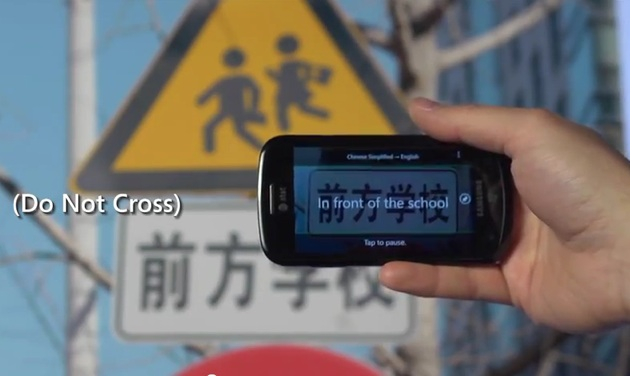
\includegraphics[width=\textwidth]{images/ocr-translator}
\end{frame}

\begin{frame}
  \frametitle{AI}
  AI (Artificial Intelligence) --- strong vs. weak.
  
  \textbf{strong AI} --- настоящий мыслящий искусственный интеллект, неотличимый от человека.
  
  \textbf{weak AI} --- штука, которая умеет выполнять некоторые когнитивные задачи, которыми обычно занимается человек.
\end{frame}

\begin{frame}
  \frametitle{Strong AI}
  \begin{center}
  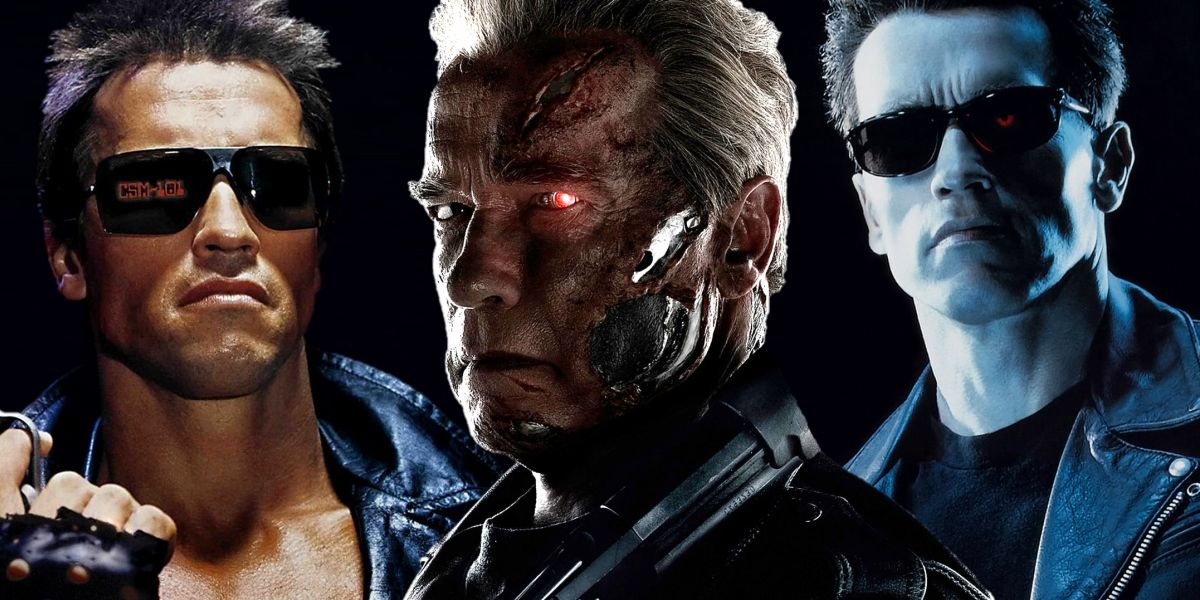
\includegraphics[width=\linewidth]{images/Terminator.jpg}
  \end{center}
\end{frame}

\begin{frame}
  \frametitle{Weak AI}
  \begin{center}
  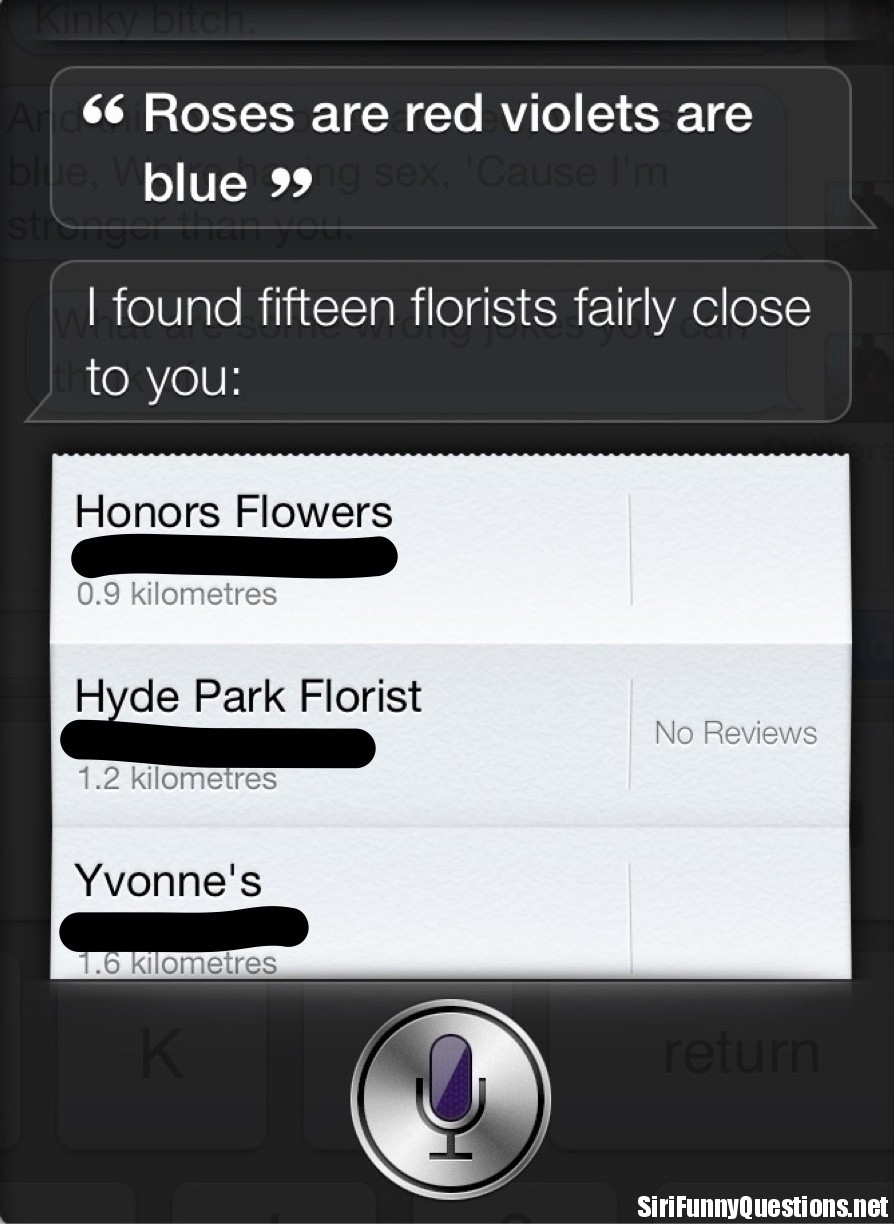
\includegraphics[height=\textheight]{images/siri.jpg}
  \end{center}
\end{frame}

\begin{frame}
  \frametitle{Weak AI}
  \begin{center}
  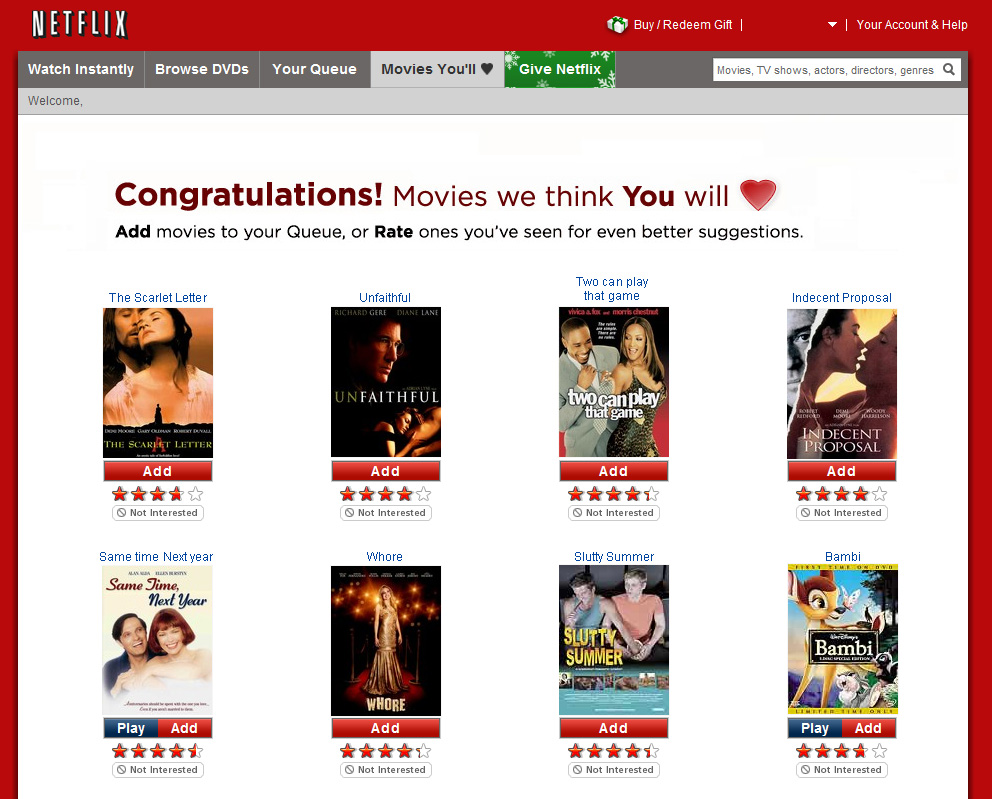
\includegraphics[width=0.9\textwidth]{images/netflix.jpg}
  \end{center}
\end{frame}

\begin{frame}
  \frametitle{Weak AI}
  \begin{center}
  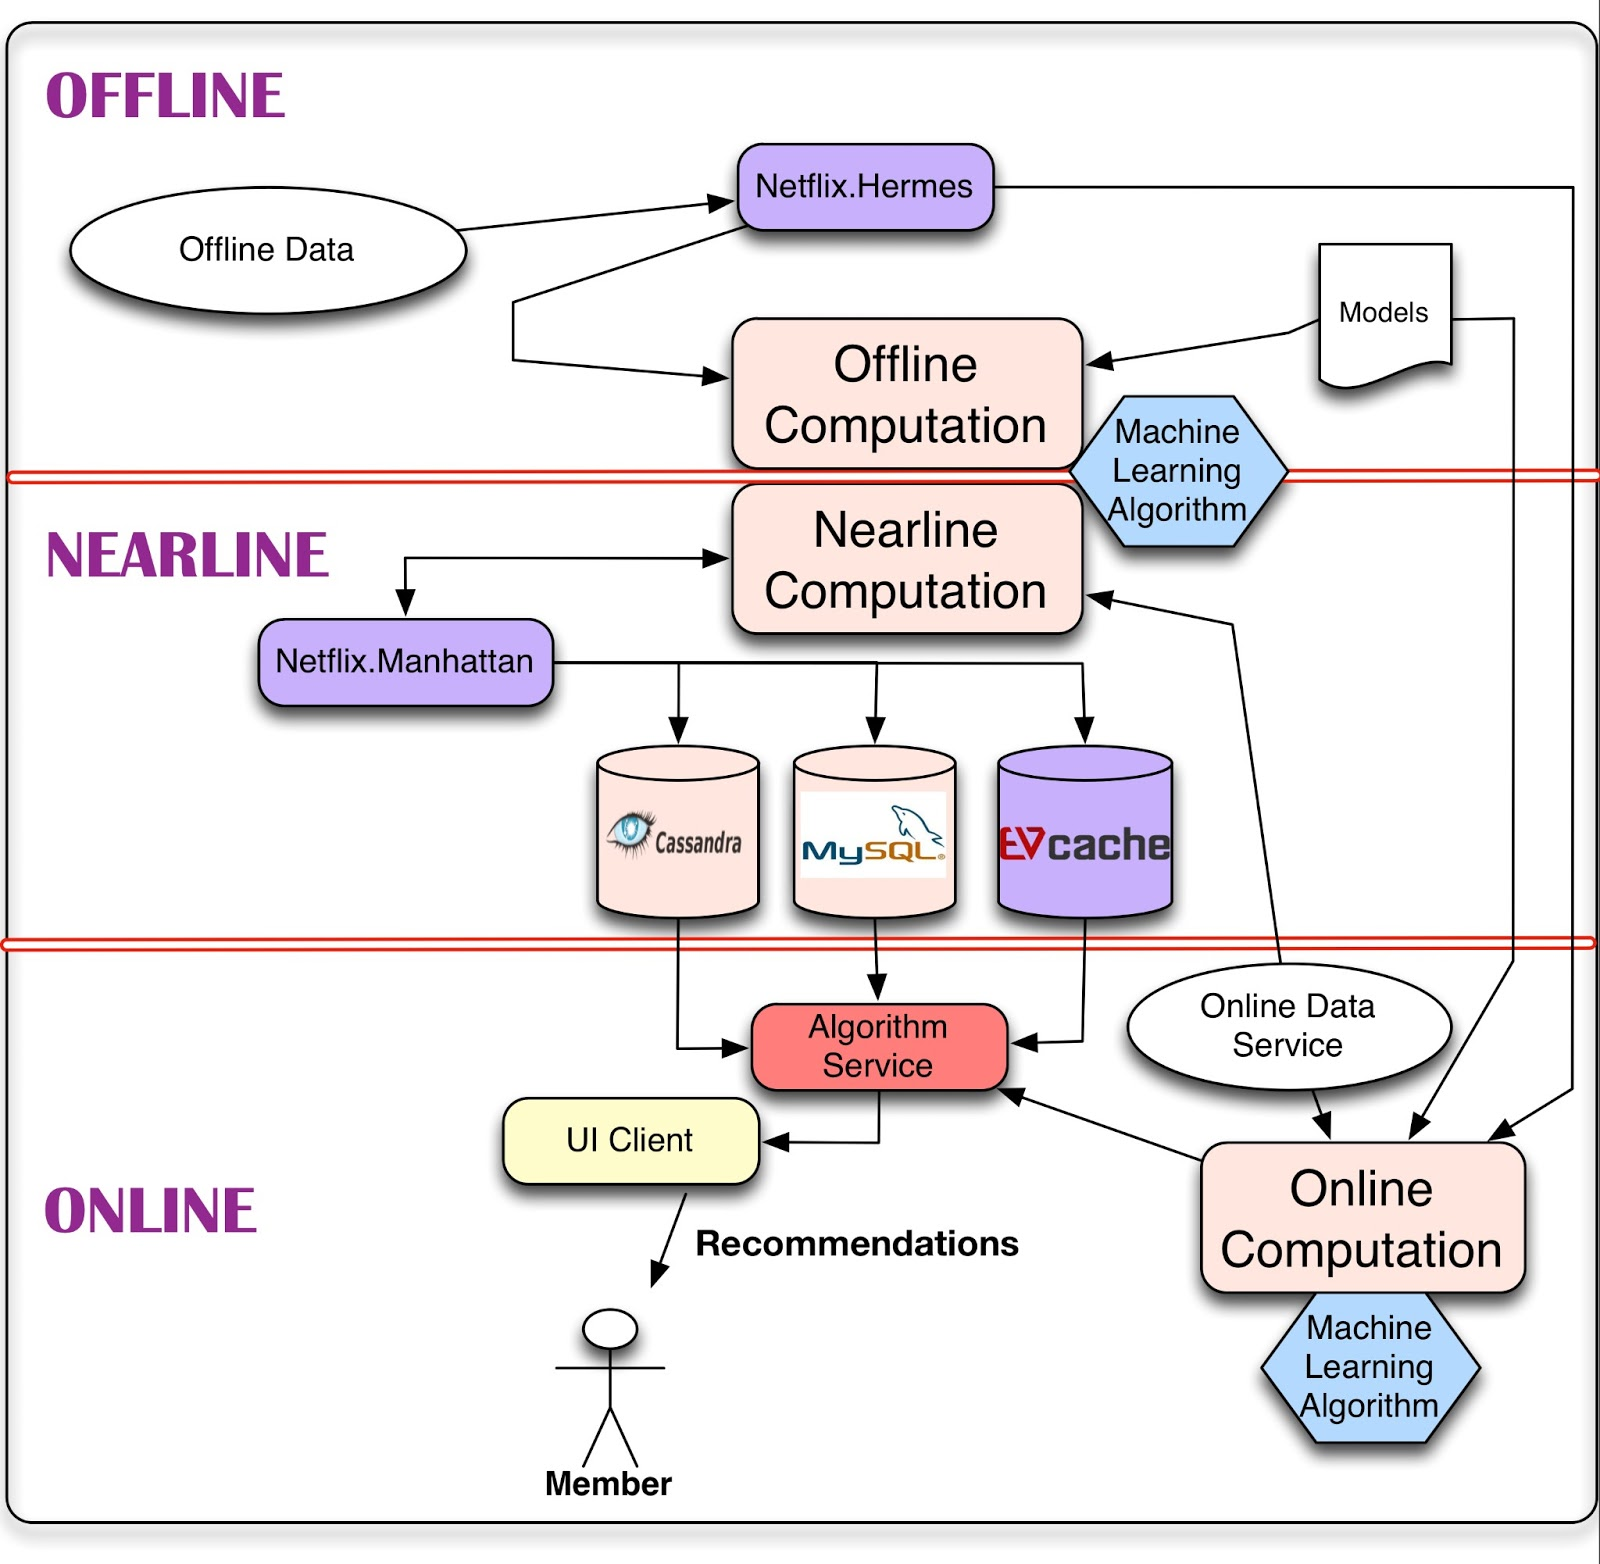
\includegraphics[height=0.9\textheight]{images/netflix.png}
  \end{center}
\end{frame}

\begin{frame}
  \frametitle{AI}
  Strong AI пока не существует, но его хотят, боятся и ищут в существующих программах при помощи теста Тьюринга.

  \alert{Что не так с тестом Тьюринга?}\\
  \vfill
  Weak AI есть вообще практически везде.
\end{frame}

\begin{frame}
  \frametitle{Нейросети}
  Нейросеть --- это магический способ решения лингвистических (и не только) проблем. Она смотрит на данные и даёт правильные (обычно) ответы на вопросы про эти данные.
  
  Только надо \sout{выбрать правильное заклинание} правильно её сконфигурировать --- это обычно самое сложное.
  
  НС используются, в частности, для speech recognition и OCR.
  
  Полным знанием о том, как работают нейросети, не обладает никто.
\end{frame}

\begin{frame}
  \frametitle{seq2seq-нейросети}
  Нейросеть вида "sequence to sequence" принимает на вход некоторую последовательность чего угодно (чисел, пикселей, символов) и порождает другую последовательность чего угодно, сооветствующую первой.
\end{frame}

\begin{frame}
  \frametitle{seq2seq-нейросети}
  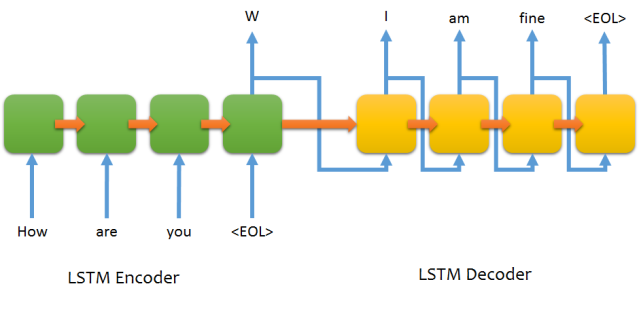
\includegraphics[width=\textwidth]{images/lstm.png}
\end{frame}

\plain{}{Cпасибо за внимание!}

\end{document}
